% Source: graduate-coursework/Sp26/CSCE763/Course_Assignments/HW3/HW3_CSCE_763_solutions.tex

\documentclass[border=4pt]{standalone}
\usepackage{amsmath}
\usepackage{amssymb}
\usepackage{graphicx}
\usepackage{tikz}
\usepackage{xcolor}
\usetikzlibrary{shapes.geometric, arrows.meta, positioning, patterns, calc}

\definecolor{USC_Garnet}{HTML}{73000A}
\definecolor{USC_Sandstorm}{HTML}{FFF2E3}
\definecolor{USC_Black90}{HTML}{363636}
\definecolor{USC_Black70}{HTML}{5C5C5C}
\definecolor{USC_Black50}{HTML}{A2A2A2}
\definecolor{USC_Black10}{HTML}{ECECEC}
\definecolor{USC_Honeycomb}{HTML}{65780B}
\definecolor{USC_Atlantic}{HTML}{466A9F}
\definecolor{USC_Congaree}{HTML}{1F414D}
\definecolor{USC_Rose}{HTML}{CC2E40}
\definecolor{USC_Grass}{HTML}{CED318}
\definecolor{USC_Horseshoe}{HTML}{65780B}
\definecolor{outputbg}{RGB}{245,245,245}

\begin{document}
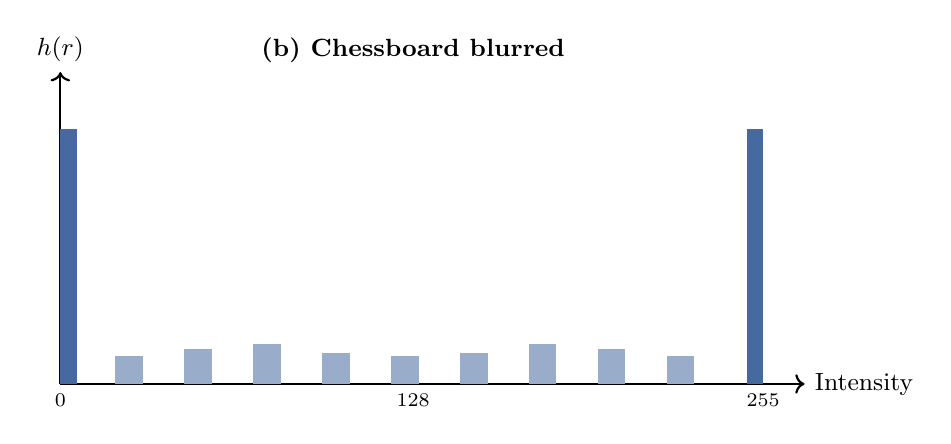
\begin{tikzpicture}[xscale=0.035, yscale=1.8]
% --- Histogram (b): Chessboard blurred ---
\begin{scope}[shift={(0,0)}]
\draw[->, thick] (0,0) -- (270,0) node[right, font=\small] {Intensity};
\draw[->, thick] (0,0) -- (0,2.2) node[above, font=\small] {$h(r)$};
\node[above, font=\small\bfseries] at (128,2.2) {(b) Chessboard blurred};
% Peaks at 0 and 255 with many intermediate levels
\fill[USC_Atlantic] (0,0) rectangle (6,1.8);
\fill[USC_Atlantic] (249,0) rectangle (255,1.8);
\fill[USC_Atlantic!55] (20,0) rectangle (30,0.2);
\fill[USC_Atlantic!55] (45,0) rectangle (55,0.25);
\fill[USC_Atlantic!55] (70,0) rectangle (80,0.28);
\fill[USC_Atlantic!55] (95,0) rectangle (105,0.22);
\fill[USC_Atlantic!55] (120,0) rectangle (130,0.2);
\fill[USC_Atlantic!55] (145,0) rectangle (155,0.22);
\fill[USC_Atlantic!55] (170,0) rectangle (180,0.28);
\fill[USC_Atlantic!55] (195,0) rectangle (205,0.25);
\fill[USC_Atlantic!55] (220,0) rectangle (230,0.2);
% Tick marks
\node[below, font=\scriptsize] at (0,0) {0};
\node[below, font=\scriptsize] at (128,0) {128};
\node[below, font=\scriptsize] at (255,0) {255};
\end{scope}
\end{tikzpicture}
\end{document}
